\documentclass[a4paper]{article}
\usepackage[a4paper, total={7in, 9in}]{geometry}
\usepackage{tikz}
\usepackage{booktabs}
\usepackage{float}
\setlength{\parindent}{0pt}
\begin{document}
\title{Requirements Management Plan Template}
\date{}
\maketitle

\textbf{Project Name:} Just-In-Time Training
\section{Planning, tracking, and reporting requirements}
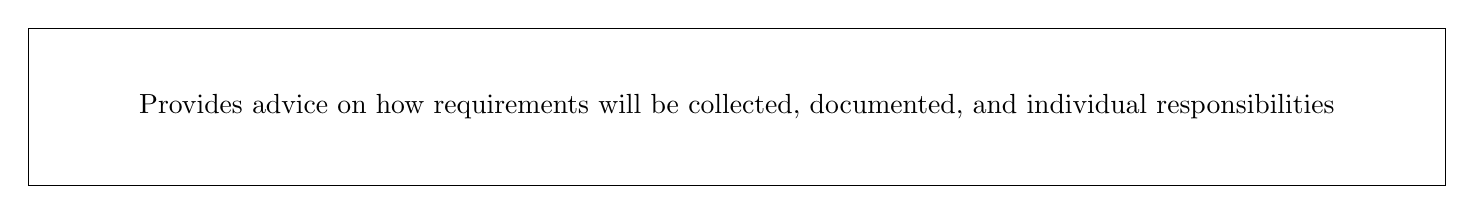
\begin{tikzpicture}
\draw (0,0) rectangle (18,2) node[pos=.5] {Provides advice on how requirements will be collected, documented, and individual responsibilities};
\end{tikzpicture}

\section{Performing configuration management activities}
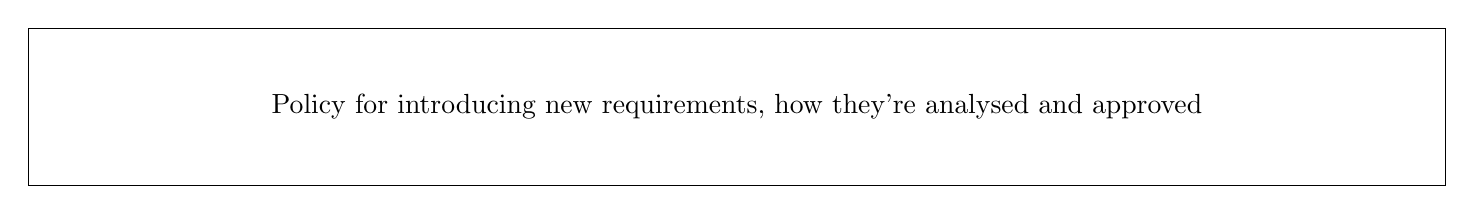
\begin{tikzpicture}
\draw (0,0) rectangle (18,2) node[pos=.5] {Policy for introducing new requirements, how they're analysed and approved};
\end{tikzpicture}

\section{Prioritising requirements}
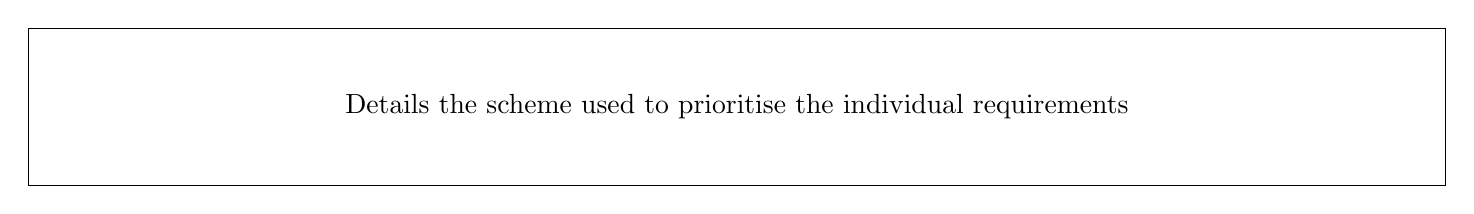
\begin{tikzpicture}
\draw (0,0) rectangle (18,2) node[pos=.5] {Details the scheme used to prioritise the individual requirements};
\end{tikzpicture}

\section{Using product metrics}
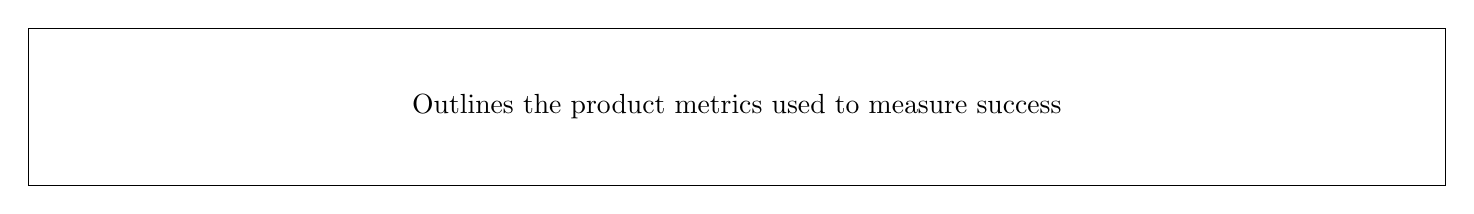
\begin{tikzpicture}
\draw (0,0) rectangle (18,2) node[pos=.5] {Outlines the product metrics used to measure success};
\end{tikzpicture}

\section{Tracing requirements}
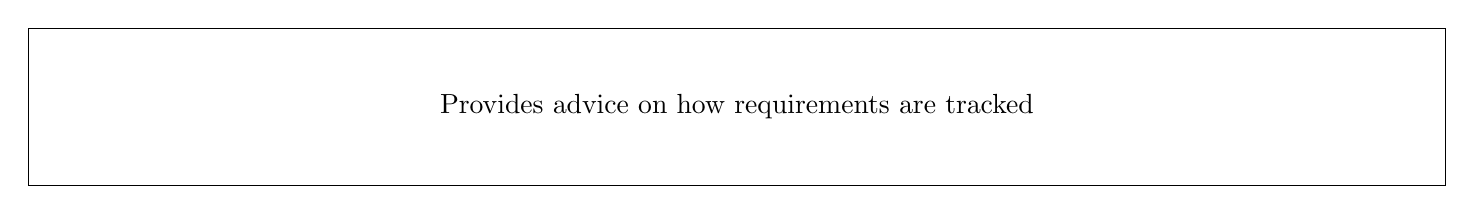
\begin{tikzpicture}
\draw (0,0) rectangle (18,2) node[pos=.5] {Provides advice on how requirements are tracked};
\end{tikzpicture}

\end{document}